\documentclass[a4paper,12pt]{article}

% ----------------------------------------------------------------
% Packages
% ----------------------------------------------------------------
\usepackage[T1]{fontenc}
\usepackage[utf8]{inputenc}
\usepackage{graphicx}
\usepackage{geometry}
\usepackage{hyperref}
\usepackage{fancyhdr}
\usepackage{xcolor}
\usepackage{listings}
\usepackage{caption}
\usepackage{booktabs}
\usepackage{enumitem}
\usepackage{verbatim}
\usepackage{float}
% 图像路径
\graphicspath{{figures/}}

% ----------------------------------------------------------------
% Page layout
% ----------------------------------------------------------------
\geometry{left=2.5cm,right=2.5cm,top=2.5cm,bottom=2.5cm}
\pagestyle{fancy}
\fancyhf{}
\rhead{POS System Report}
\lhead{Software Engineering Practice}
\cfoot{\thepage}

% ----------------------------------------------------------------
% Listings configuration
% ----------------------------------------------------------------
\lstdefinestyle{mystyle}{
  backgroundcolor=\color{gray!10},
  commentstyle=\color{green!50!black},
  keywordstyle=\color{blue!70!black},
  numberstyle=\tiny\color{gray},
  stringstyle=\color{orange!70!black},
  basicstyle=\ttfamily\small,
  breakatwhitespace=false,
  breaklines=true,
  captionpos=b,
  keepspaces=true,
  numbers=left,
  numbersep=5pt,
  showspaces=false,
  showstringspaces=false,
  showtabs=false,
  tabsize=2
}
\lstset{style=mystyle}

% ----------------------------------------------------------------
% Title
% ----------------------------------------------------------------
\title{Part~2 -- Implementation Report\\Point-of-Sale (POS) System}
\author{Group XXX: Member~A \and Member~B \and Member~C}
\date{\today}

\begin{document}
\maketitle
\tableofcontents
\newpage

% ----------------------------------------------------------------
\section{Introduction}
This report documents the implementation phase of our Point-of-Sale (POS) system, developed as the second part of the \emph{Software Engineering Practice} assignment.  
The project demonstrates the application of Object-Oriented (OO) analysis, design and implementation techniques, supported by modern version-control practices with Git and GitHub.

Core objectives were:
\begin{itemize}[nosep]
  \item Provide a working POS application capable of \textbf{processing sales} and \textbf{handling returns}.\footnote{Both CLI and GUI front-ends are available.}
  \item Apply a \textbf{three-layer architecture} (UI, Service, Domain) with clear separation of concerns.
  \item Employ OO principles (abstraction, encapsulation, inheritance, polymorphism) and relevant design patterns (Service Layer, Domain Model).
  \item Maintain full team collaboration through feature branches, pull-requests and documented Git history.
\end{itemize}

% ----------------------------------------------------------------
\section{System Overview}
\subsection{Use Case Model}
Figure~\ref{fig:use-case} shows the Use Case Diagram for the POS system. The two primary use cases required by the assignment are \textbf{Process Sale} and \textbf{Handle Returns}.

\begin{figure}[H]
  \centering
  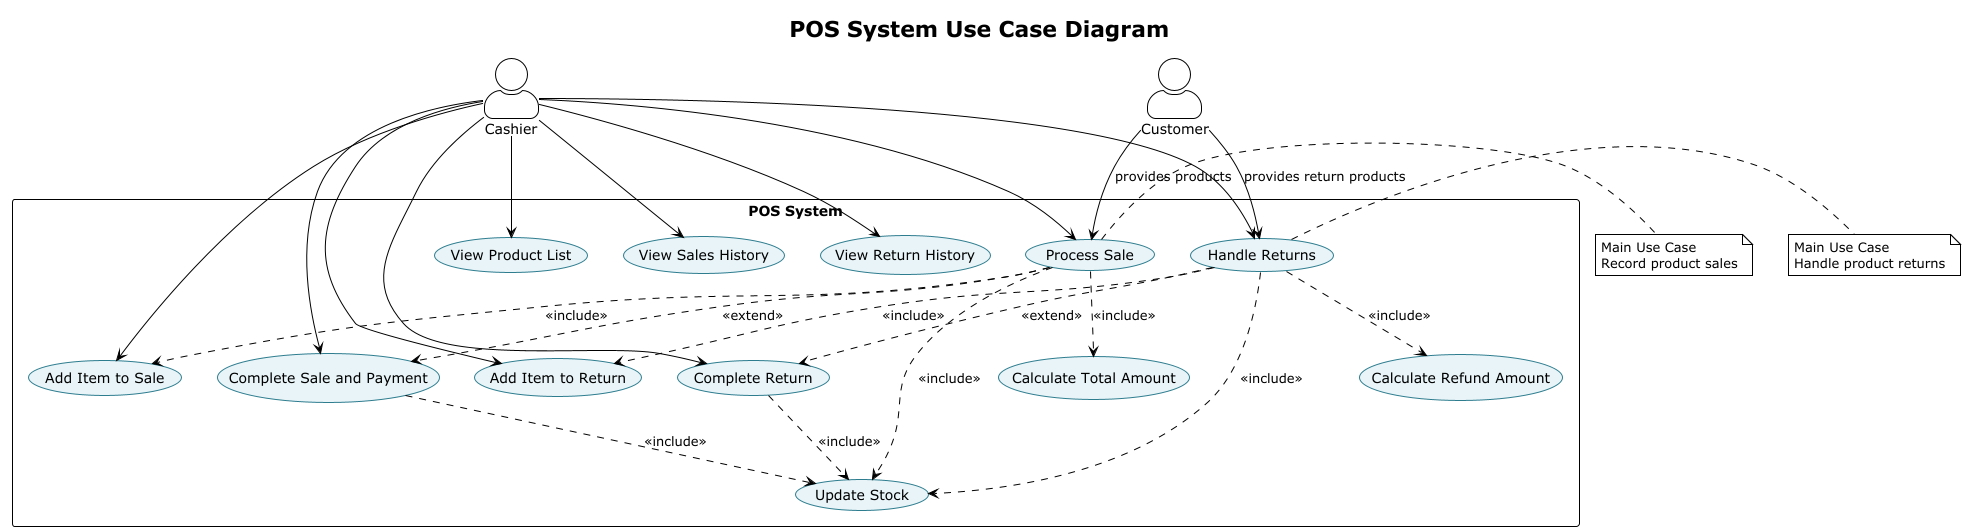
\includegraphics[width=0.95\textwidth]{Use_Case_Diagram-POS_System.png}
  \caption{Use Case Diagram of the POS System}
  \label{fig:use-case}
\end{figure}

\subsection{Architecture}
The system adopts a three-layer logical architecture. Figure~\ref{fig:architecture} presents the package/module organisation used in implementation, which helps separate UI, service logic, and domain model concerns.

\begin{figure}[H]
  \centering
  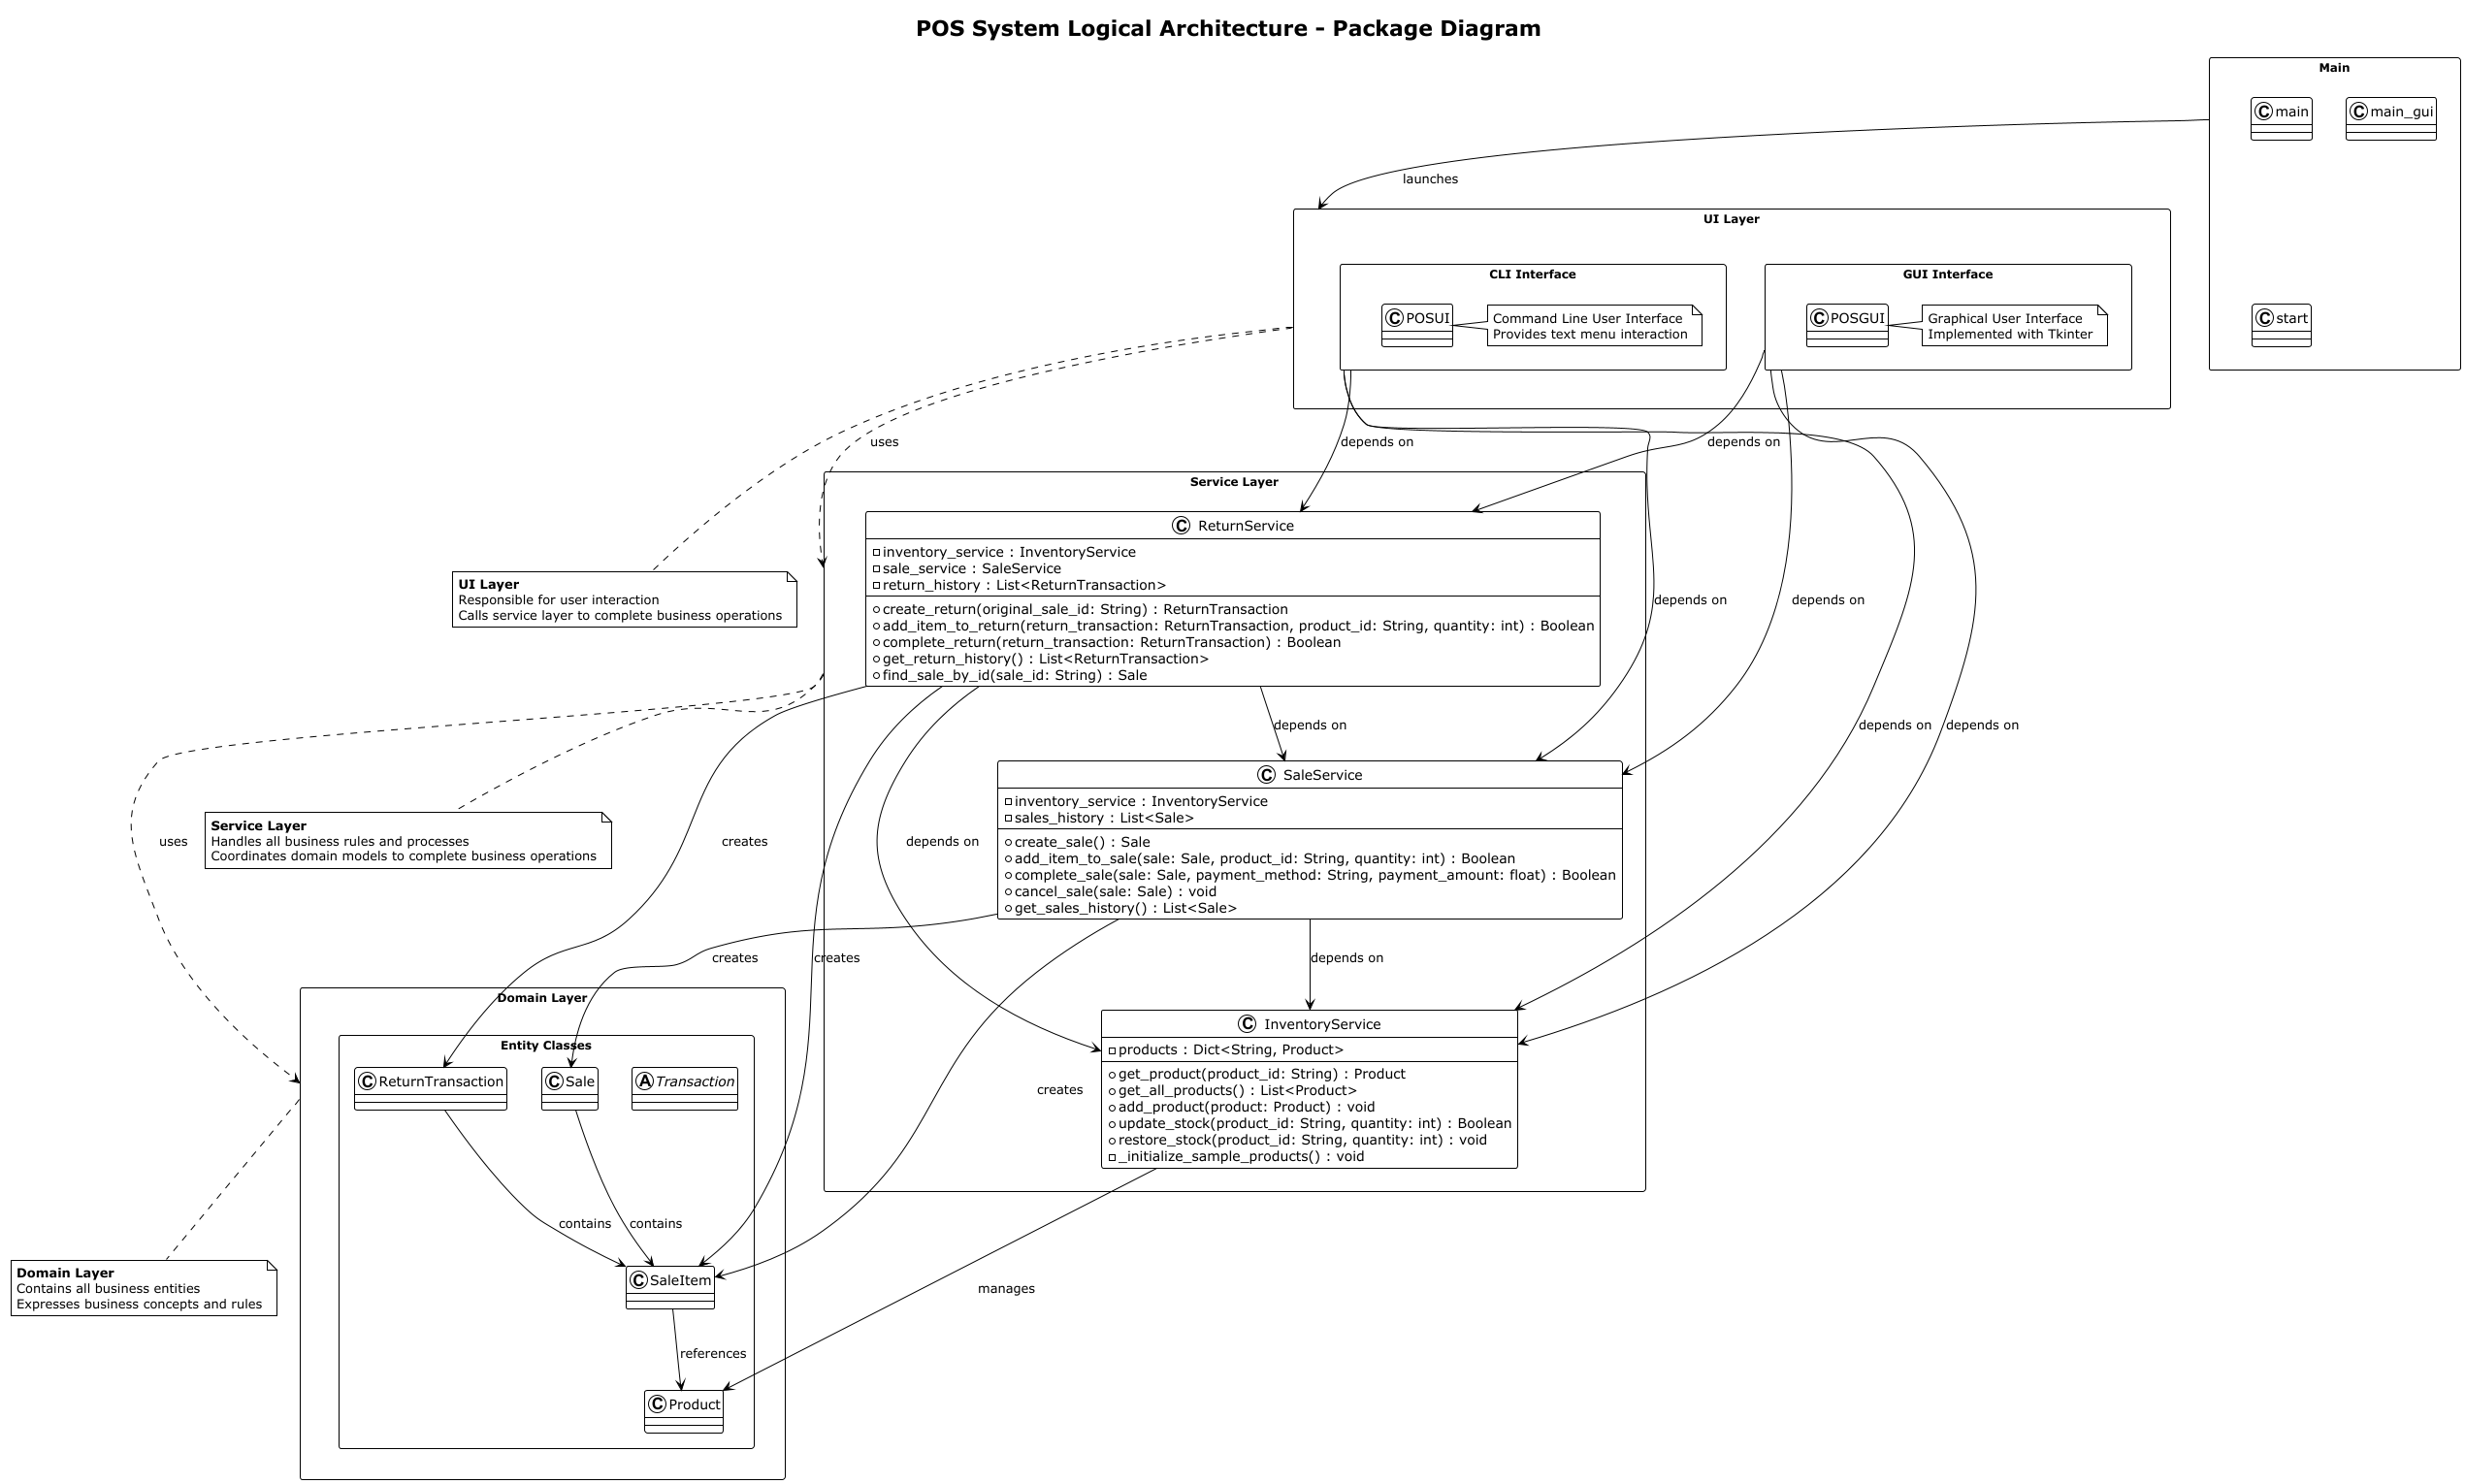
\includegraphics[width=0.95\textwidth]{Logical_Architecture_Package_Diagram-POS_System.png}
  \caption{Logical Architecture Package Diagram}
  \label{fig:architecture}
\end{figure}

\subsection{Domain Model}
Key business entities appear in the domain layer (Figure~\ref{fig:domain-model}). They are implemented in the \texttt{domain/} package and form the backbone of the application logic.

\begin{figure}[H]
  \centering
  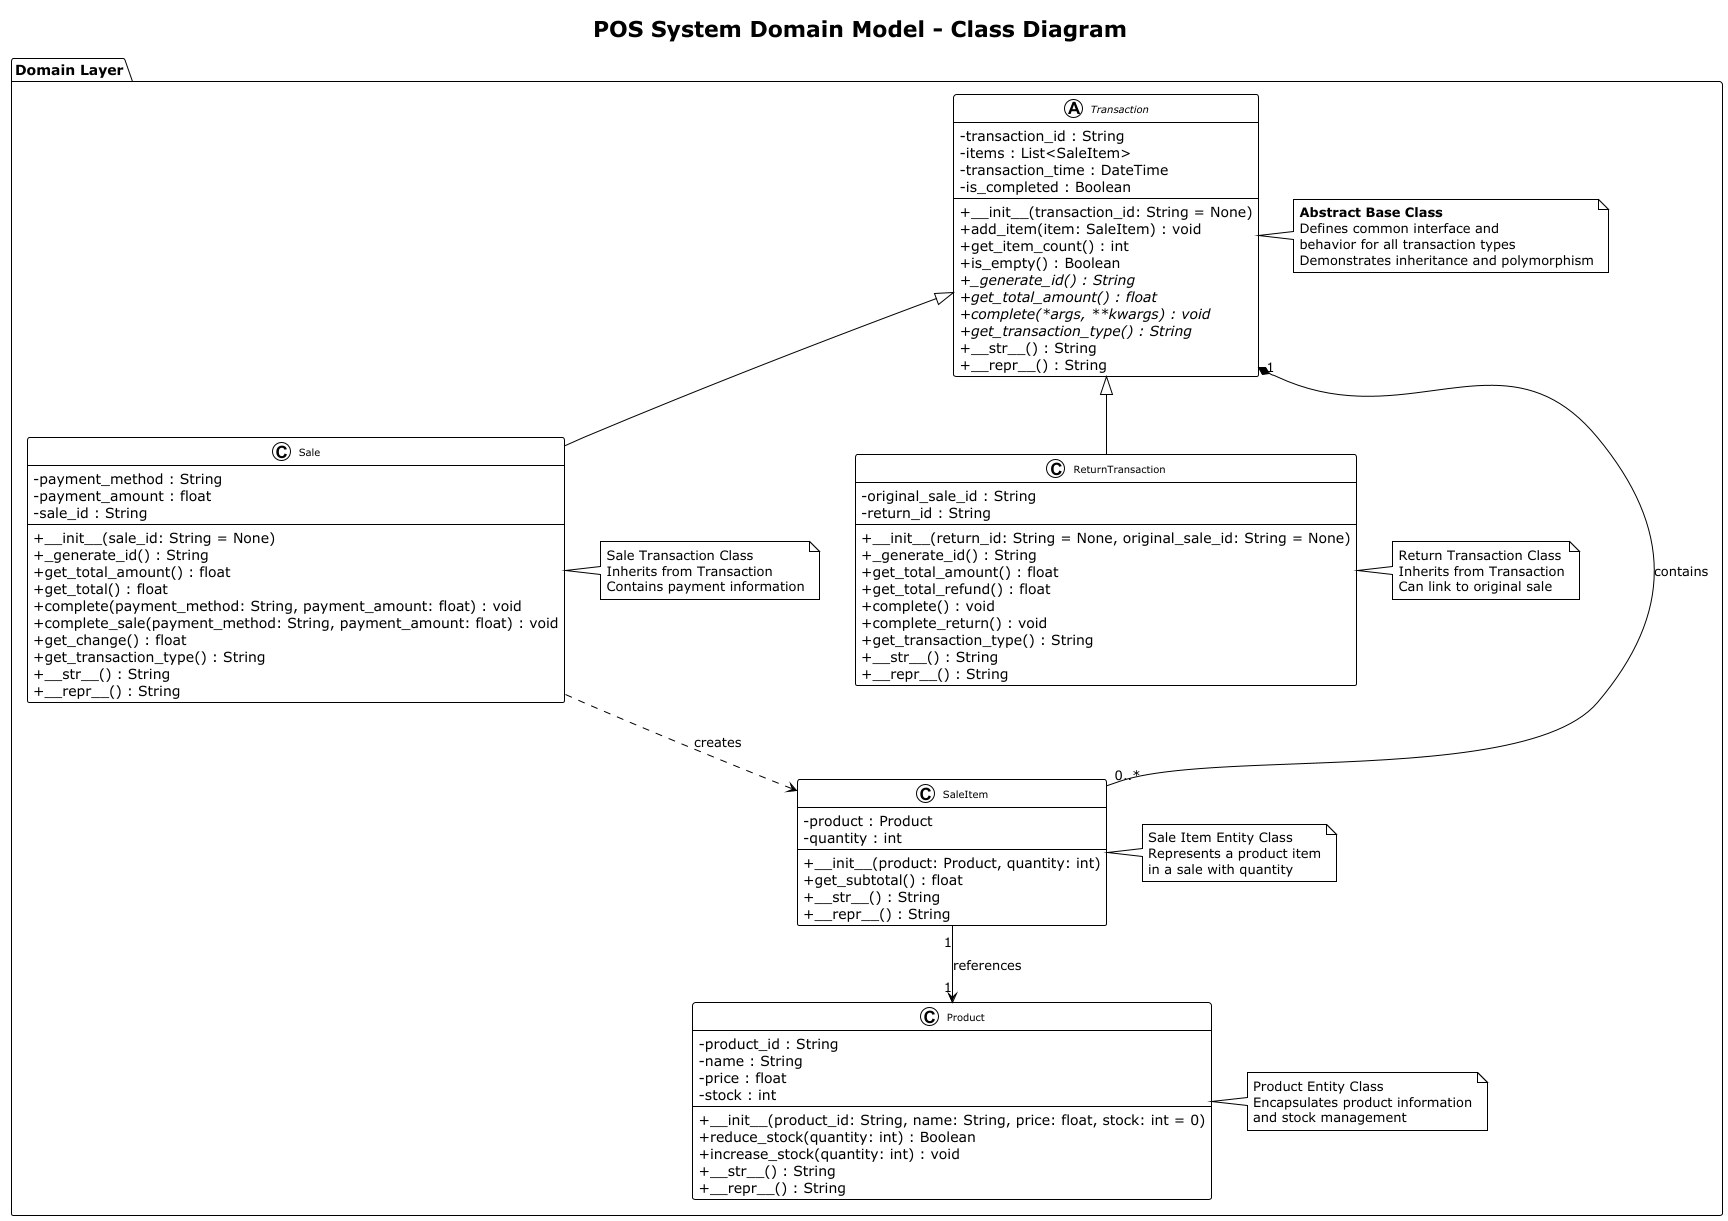
\includegraphics[width=0.95\textwidth]{Domain_Model_Class_Diagram-POS_System.png}
  \caption{Domain Model Class Diagram}
  \label{fig:domain-model}
\end{figure}

% ----------------------------------------------------------------
\section{System Development}
\subsection{Tasks Completed}
Table1 summarises the functional and documentation artefacts delivered.

\begin{table}[H]
  \centering
  \begin{tabular}{p{0.35\textwidth}p{0.55\textwidth}}
    \toprule
    \textbf{Category} & \textbf{Deliverables} \\
    \midrule
    Project Structure & Three-layer package skeleton (\texttt{domain/}, \texttt{service/}, \texttt{ui/}) \\
    Domain Layer & \texttt{Product}, \texttt{Sale}, \texttt{SaleItem}, \texttt{ReturnTransaction} \\
    Service Layer & \texttt{InventoryService}, \texttt{SaleService}, \texttt{ReturnService} \\
    UI Layer & CLI (\texttt{pos\_ui.py}), GUI (\texttt{pos\_gui.py}) built with Tkinter \\
    Core Use-Cases & Process Sale, Handle Returns (end-to-end) \\
    Persistence & In-memory store; interface prepared for future DB layer \\
    Tests & \texttt{test\_pos\_system.py} unit / integration tests \\
    UML Artefacts & Use-Case diagram, SSDs, Domain Class diagram, Package diagram, Interaction diagrams (PlantUML) \\
    Documentation & README, ARCHITECTURE, PROJECT\_SUMMARY, this Report \\
    \bottomrule
  \end{tabular}
  \caption{Summary of completed development tasks}
  \label{tab:tasks}
\end{table}

\subsection{Interaction Diagrams}
To illustrate the dynamic behaviour of key use cases, we include two sequence diagrams generated with PlantUML.

\begin{figure}[H]
  \centering
  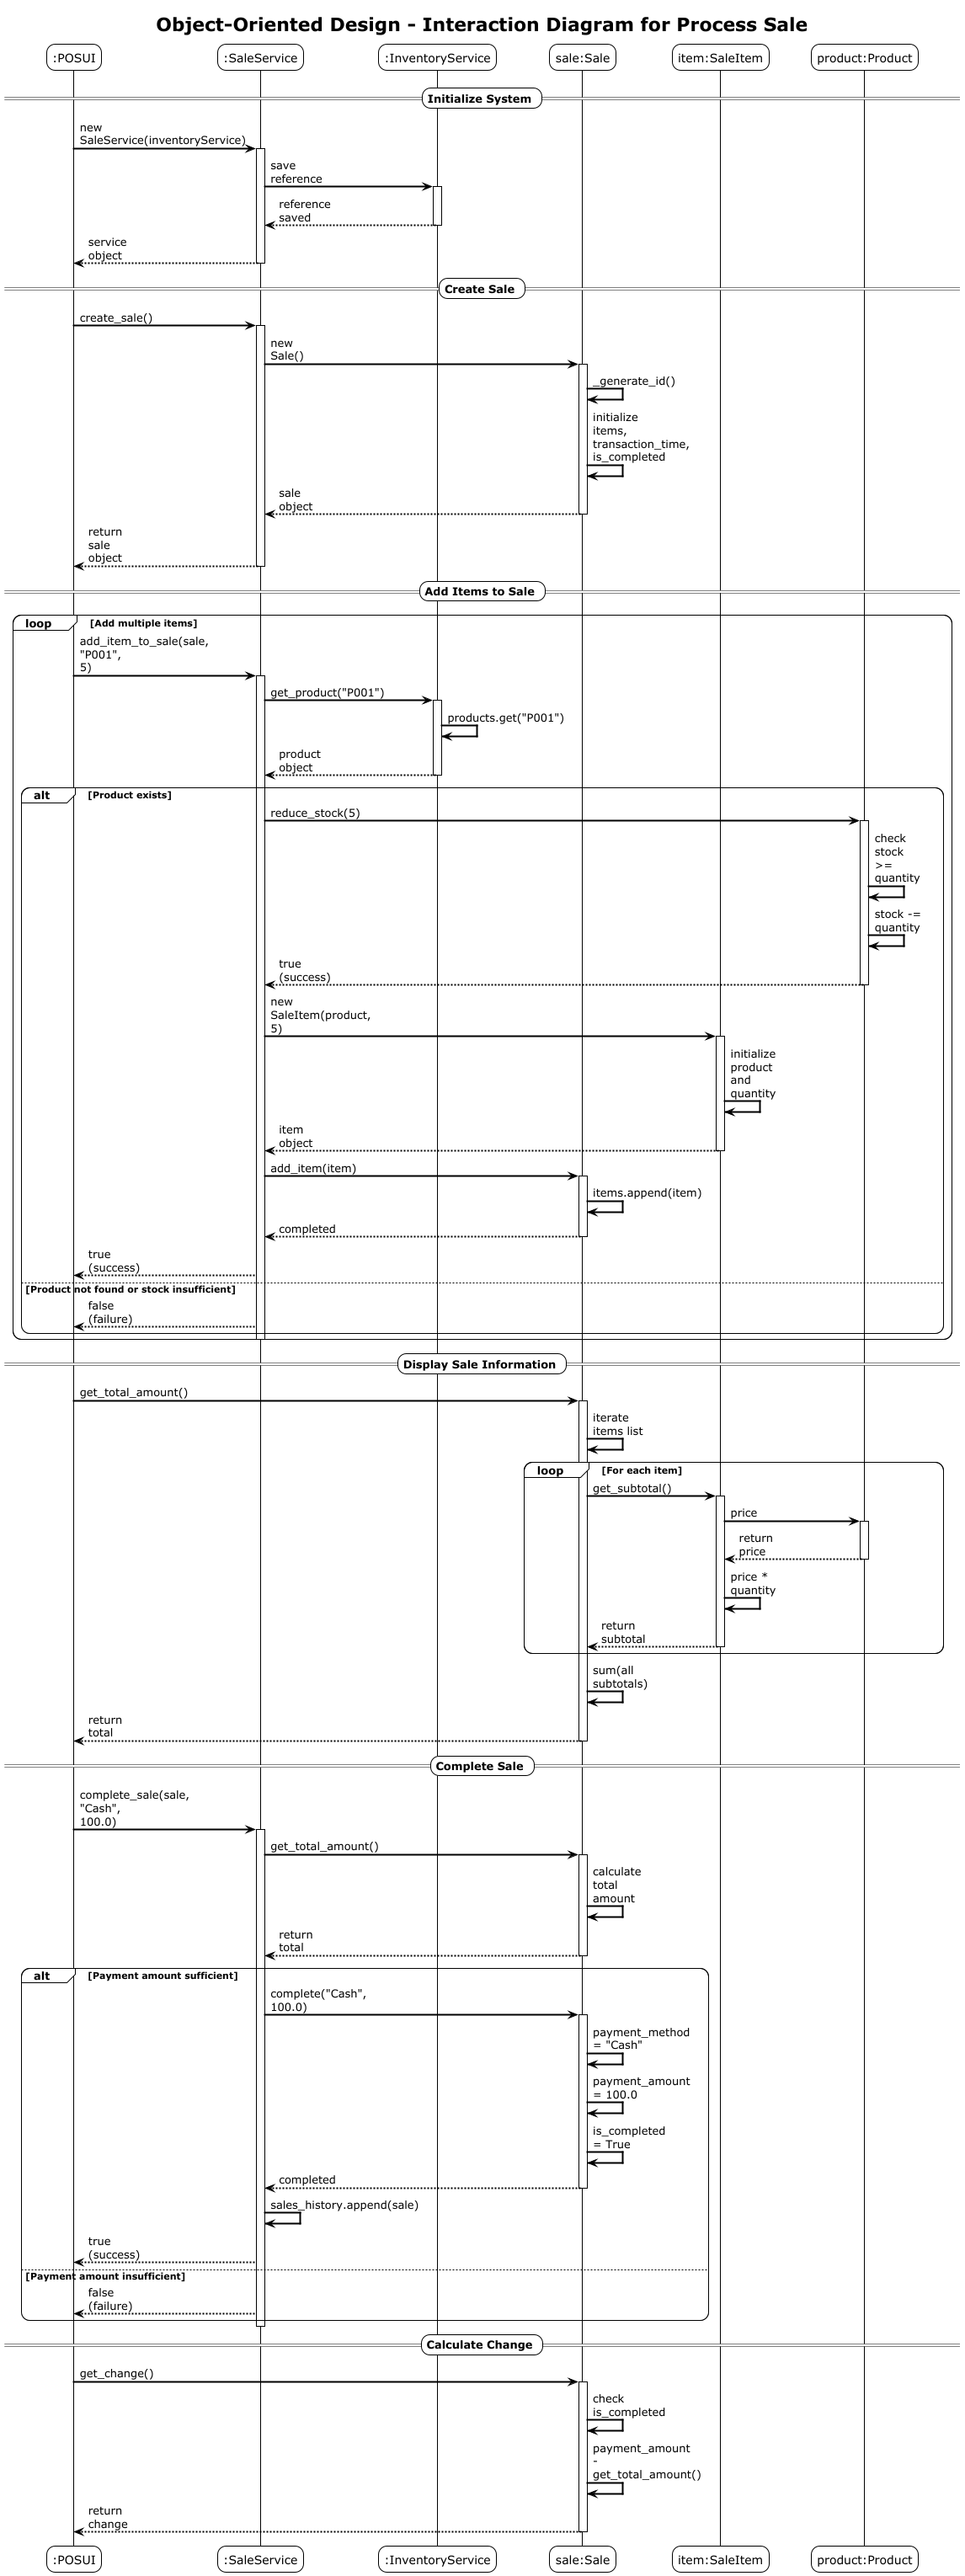
\includegraphics[width=0.6\textwidth]{OO_Design_Interaction_Diagram___Process_Sale-Object.png}
  \caption{Interaction Diagram – Process Sale}
\end{figure}

\begin{figure}[H]
  \centering
  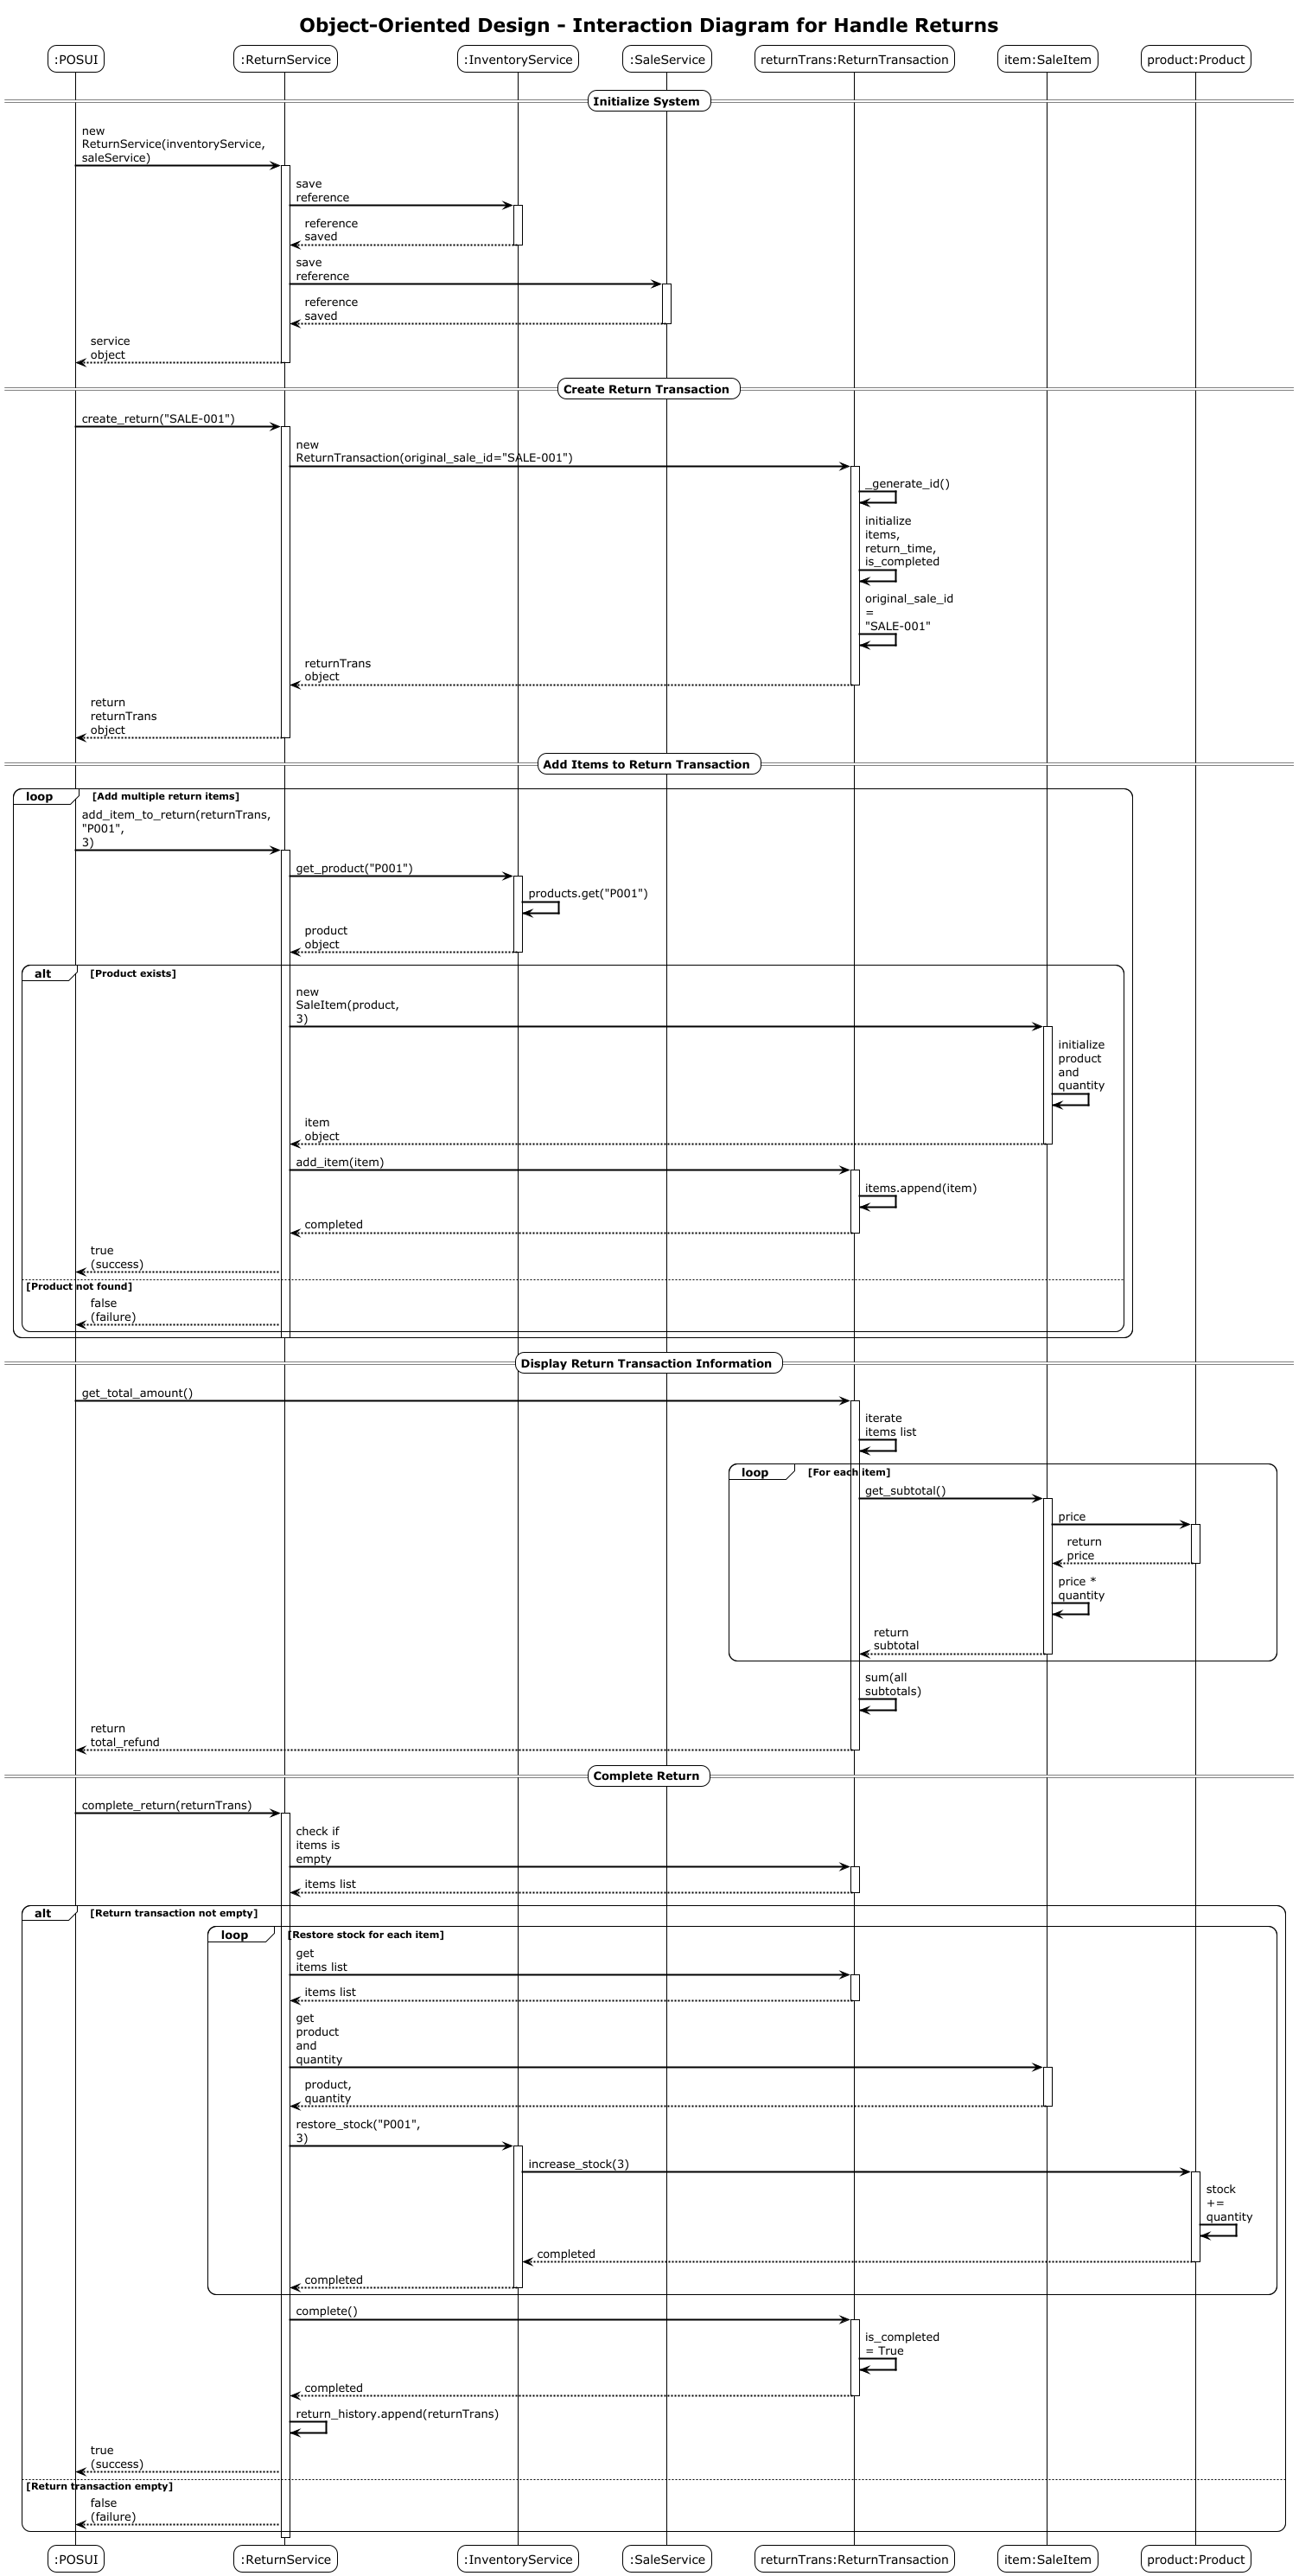
\includegraphics[width=0.7\textwidth]{OO_Design_Interaction_Diagram___Handle_Returns-Object.png}
  \caption{Interaction Diagram – Handle Returns}
\end{figure}
% ----------------------------------------------------------------
\section{Implementation Snippets}
Rather than embedding the entire code-base, representative excerpts are included using \verb|lstinputlisting|.  Full source is available in the repository.

\subsection{Domain Layer}
\lstinputlisting[language=Python,caption={Transaction Abstract Class},label={lst:transaction}]{../../domain/transaction.py}

\lstinputlisting[language=Python,caption={Sale Entity Class},label={lst:sale}]{../../domain/sale.py}

\subsection{Service Layer}
\lstinputlisting[language=Python,caption={Inventory Service},label={lst:inventory}]{../../service/inventory_service.py}

\lstinputlisting[language=Python,caption={Sale Service},label={lst:sale-service}]{../../service/sale_service.py}

% ----------------------------------------------------------------
\section{Git Command History}
Team collaboration was fully tracked in GitHub. A condensed commit log covering all branches is embedded below (generated on \today):

\begin{verbatim}
% Run in repo root:
%   git log --graph --oneline --all --decorate --since=2025-01-01 > docs/report/git_history.txt
\end{verbatim}

\vspace{0.5em}
% Uncomment when file is present
%\verbatiminput{git_history.txt}

% ----------------------------------------------------------------
\section{Screenshots}
This section provides an overview of the POS system's graphical user interface. The screenshots highlight the main workflow screens (sales and returns), supporting views (product list), and the transaction history used to verify completed operations.

\begin{figure}[H]
  \centering
  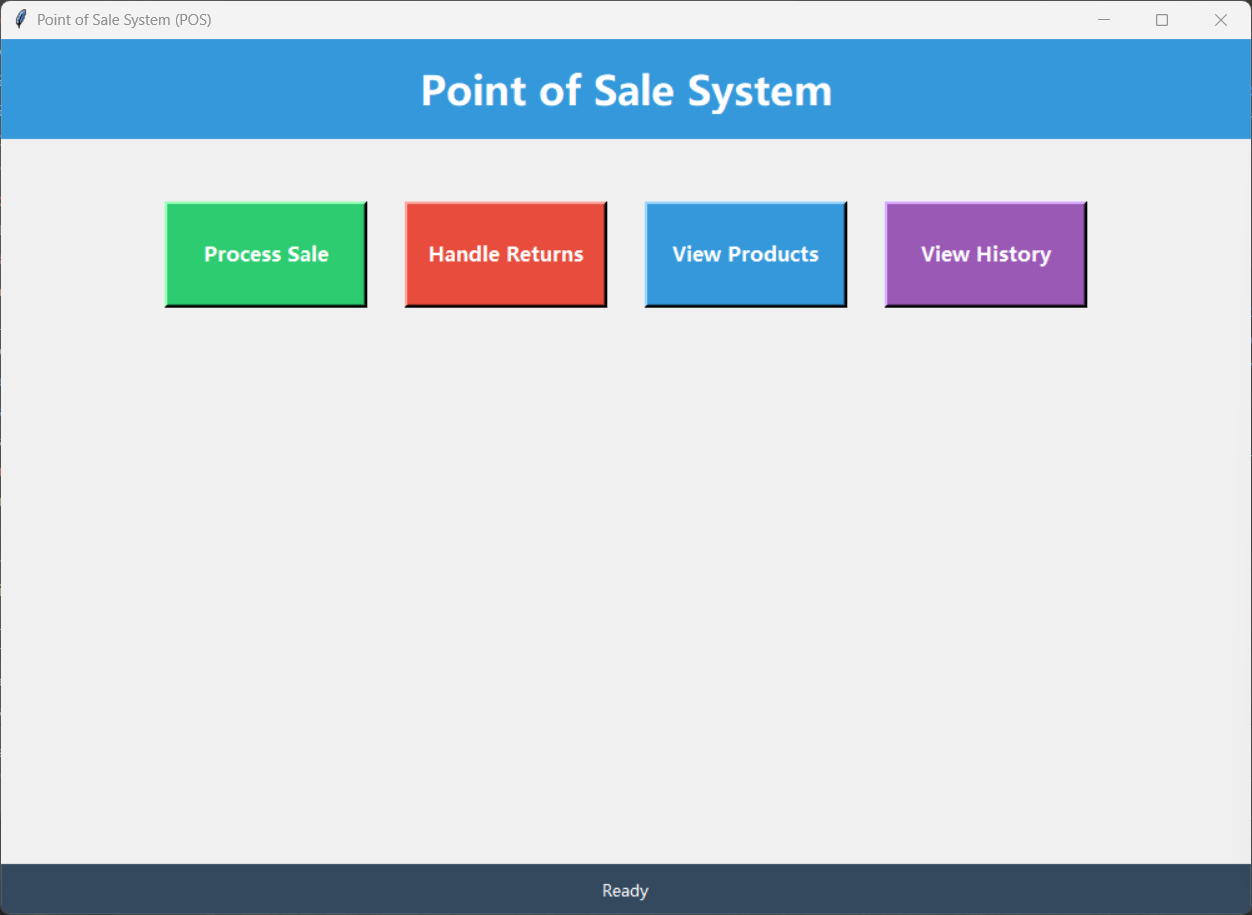
\includegraphics[width=0.9\textwidth]{main_menu.png}
  \caption{Main Menu}
\end{figure}

\begin{figure}[H]
  \centering
  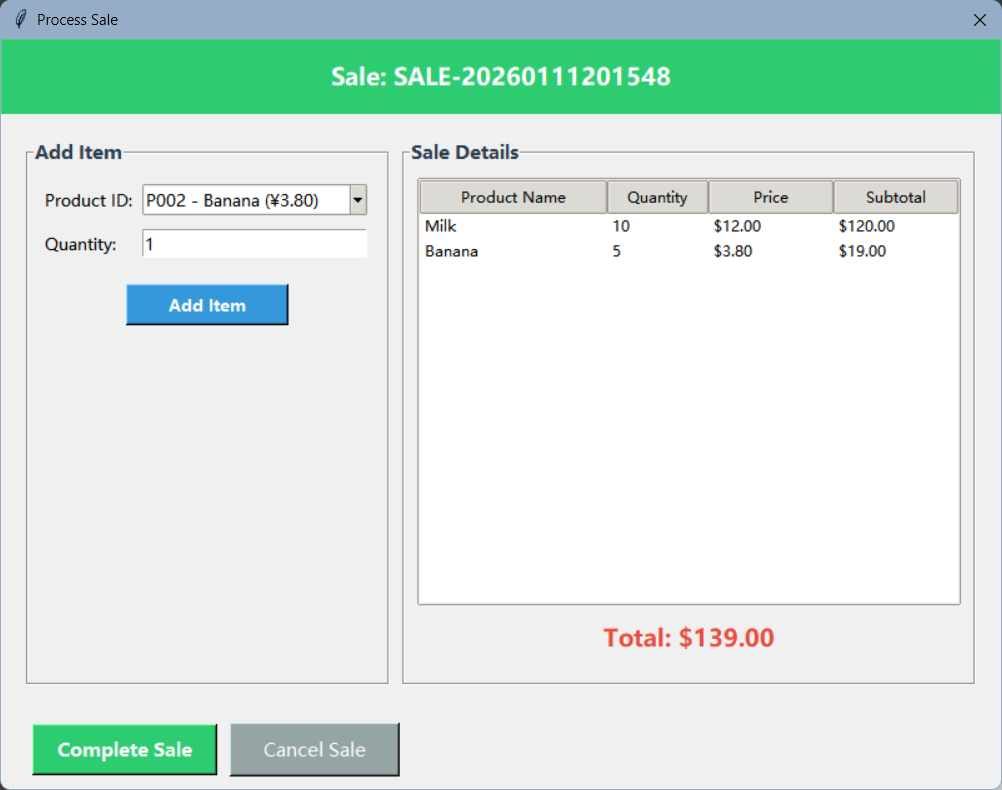
\includegraphics[width=0.9\textwidth]{sale_page.png}
  \caption{Process Sale Screen}
\end{figure}

\begin{figure}[H]
  \centering
  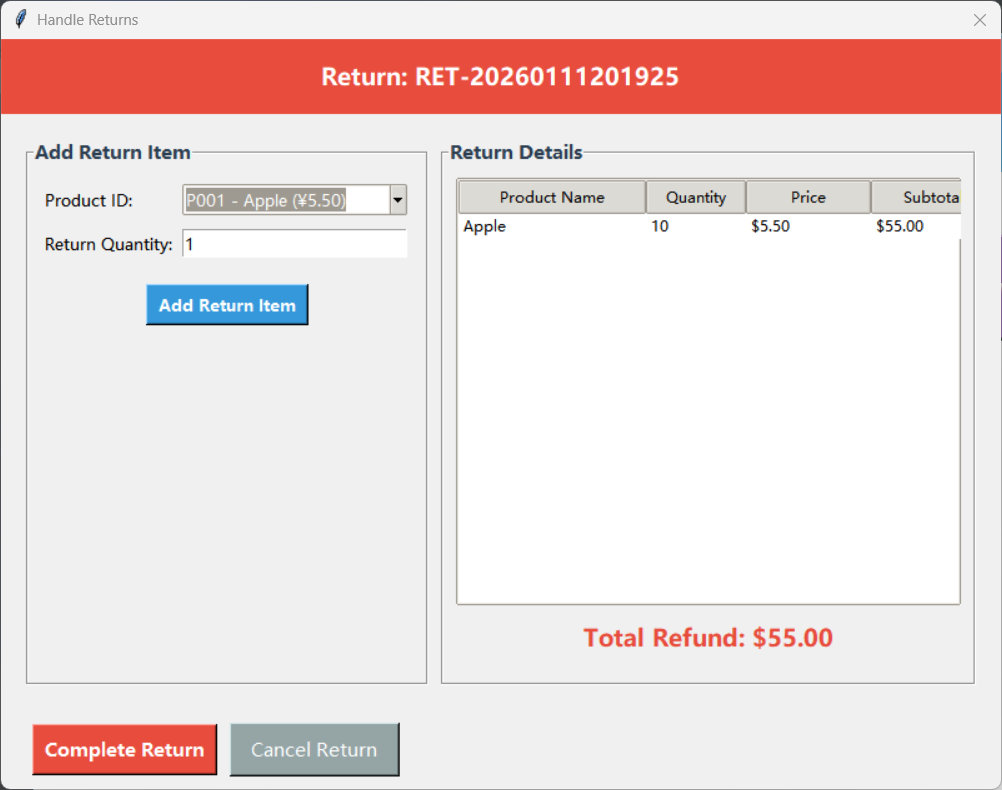
\includegraphics[width=0.9\textwidth]{return_page.png}
  \caption{Handle Returns Screen}
\end{figure}

\begin{figure}[H]
  \centering
  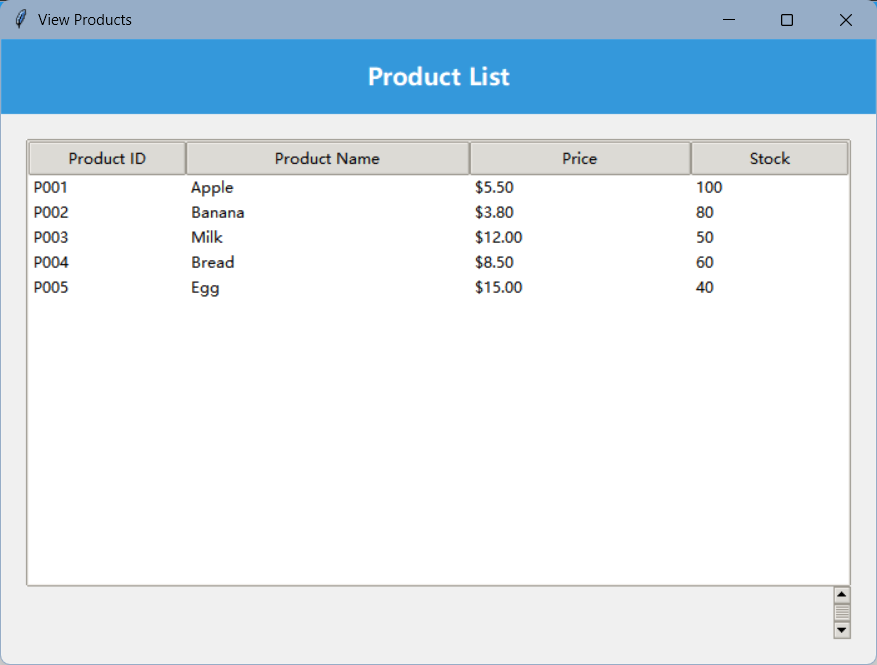
\includegraphics[width=0.9\textwidth]{product_list.png}
  \caption{Product List Screen}
\end{figure}

\begin{figure}[H]
  \centering
  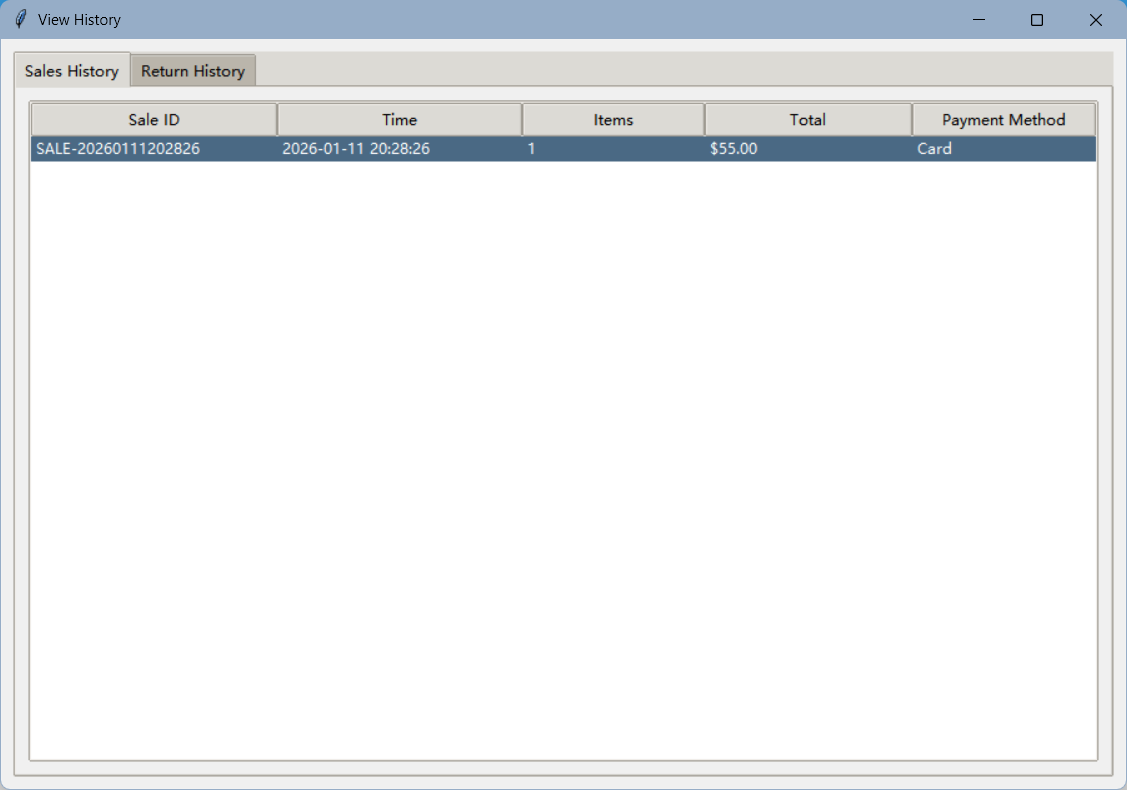
\includegraphics[width=0.9\textwidth]{history.png}
  \caption{Sales and Returns History Screen}
\end{figure}

% ----------------------------------------------------------------
\section{Conclusion}
The project successfully delivered a functional POS system demonstrating complete OO lifecycle coverage—from requirements modelling through to working software and documentation.
Key take-aways include:
\begin{itemize}[nosep]
  \item The three-layer architecture proved effective in separating UI, service logic and domain concerns.
  \item PlantUML integrated smoothly into the documentation workflow, enabling living UML diagrams.
  \item Collective code ownership was facilitated by strict branch discipline and frequent merges, resulting in minimal integration conflicts.
\end{itemize}
Future work may integrate persistent storage, extend reporting capabilities and introduce fine-grained user authentication.

\end{document}

